\documentclass[
  bibliography=totoc,     % Literatur im Inhaltsverzeichnis
  captions=tableheading,  % Tabellenüberschriften
  titlepage=firstiscover, % Titelseite ist Deckblatt
]{scrartcl}

% Paket float verbessern
\usepackage{scrhack}

% Warnung, falls nochmal kompiliert werden muss
\usepackage[aux]{rerunfilecheck}

% unverzichtbare Mathe-Befehle
\usepackage{amsmath}
% viele Mathe-Symbole
\usepackage{amssymb}
% Erweiterungen für amsmath
\usepackage{mathtools}

% Fonteinstellungen
\usepackage{fontspec}
% Latin Modern Fonts werden automatisch geladen
% Alternativ zum Beispiel:
%\setromanfont{Libertinus Serif}
%\setsansfont{Libertinus Sans}
%\setmonofont{Libertinus Mono}

% Wenn man andere Schriftarten gesetzt hat,
% sollte man das Seiten-Layout neu berechnen lassen
\recalctypearea{}

% deutsche Spracheinstellungen
\usepackage[ngerman]{babel}


\usepackage[
  math-style=ISO,    % ┐
  bold-style=ISO,    % │
  sans-style=italic, % │ ISO-Standard folgen
  nabla=upright,     % │
  partial=upright,   % │
  mathrm=sym,        % ┘
  warnings-off={           % ┐
    mathtools-colon,       % │ unnötige Warnungen ausschalten
    mathtools-overbracket, % │
  },                       % ┘
]{unicode-math}

% traditionelle Fonts für Mathematik
\setmathfont{Latin Modern Math}
% Alternativ zum Beispiel:
%\setmathfont{Libertinus Math}

\setmathfont{XITS Math}[range={scr, bfscr}]
\setmathfont{XITS Math}[range={cal, bfcal}, StylisticSet=1]

% Zahlen und Einheiten
\usepackage[
  locale=DE,                   % deutsche Einstellungen
  separate-uncertainty=true,   % immer Unsicherheit mit \pm
  per-mode=symbol-or-fraction, % / in inline math, fraction in display math
]{siunitx}

% chemische Formeln
\usepackage[
  version=4,
  math-greek=default, % ┐ mit unicode-math zusammenarbeiten
  text-greek=default, % ┘
]{mhchem}

% richtige Anführungszeichen
\usepackage[autostyle]{csquotes}

% schöne Brüche im Text
\usepackage{xfrac}

% Standardplatzierung für Floats einstellen
\usepackage{float}
\floatplacement{figure}{htbp}
\floatplacement{table}{htbp}

% Floats innerhalb einer Section halten
\usepackage[
  section, % Floats innerhalb der Section halten
  below,   % unterhalb der Section aber auf der selben Seite ist ok
]{placeins}

% Seite drehen für breite Tabellen: landscape Umgebung
\usepackage{pdflscape}

% Captions schöner machen.
\usepackage[
  labelfont=bf,        % Tabelle x: Abbildung y: ist jetzt fett
  font=small,          % Schrift etwas kleiner als Dokument
  width=0.9\textwidth, % maximale Breite einer Caption schmaler
]{caption}
% subfigure, subtable, subref
\usepackage{subcaption}

% Grafiken können eingebunden werden
\usepackage{graphicx}

% schöne Tabellen
\usepackage{tabularray}
\UseTblrLibrary{booktabs, siunitx}

% Verbesserungen am Schriftbild
\usepackage{microtype}

% Literaturverzeichnis
\usepackage[
  backend=biber,
]{biblatex}
% Quellendatenbank
\addbibresource{lit.bib}
\addbibresource{programme.bib}

% Hyperlinks im Dokument
\usepackage[
  german,
  unicode,        % Unicode in PDF-Attributen erlauben
  pdfusetitle,    % Titel, Autoren und Datum als PDF-Attribute
  pdfcreator={},  % ┐ PDF-Attribute säubern
  pdfproducer={}, % ┘
]{hyperref}
% erweiterte Bookmarks im PDF
\usepackage{bookmark}

% Trennung von Wörtern mit Strichen
\usepackage[shortcuts]{extdash}

\author{%
  Vincent Wirsdörfer\\%
  \href{mailto:vincent.wirsdoerfer@udo.edu}{authorA@udo.edu}%
  \and%
  Joris Daus\\%
  \href{mailto:joris.daus@udo.edu}{authorB@udo.edu}%
}
\publishers{TU Dortmund – Fakultät Physik}


\begin{document}


\section{Versuchsdurchführung}
\label{sec:Versuchsdurchfuehrung}

Zu Beginn des Experiments werden die geometrischen Maße der vorliegenden Versuchsmaterialien gesammelt. Hierzu 
werden jeweils die Dicken der Drähte und der Folien aller metallischer Proben gemessen. Die Längen der Spulendrähte
von Kupfer, Silber und Tantal können abgelesen werden.\\

\noindent Im Folgenden werden die elektrischen Widerstände der Metalle aufgenommen. Dazu wird die untenstehende Abbildung 
nachgebaut.

\begin{figure}
    \centering
    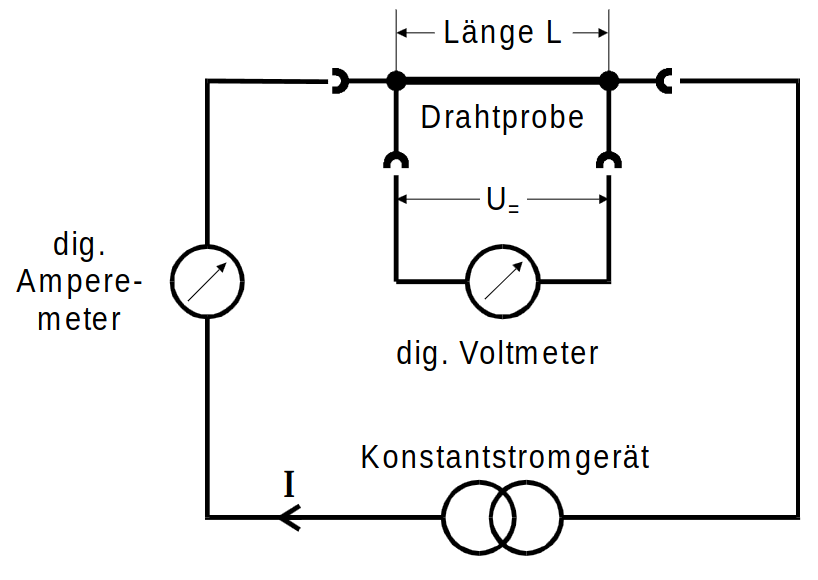
\includegraphics[height=6cm]{Widerstand.png}
    \caption{Messung der Drahtwiderstände \cite{Versuchsanleitung_v511}.}
    \label{fig:Widerstand}
\end{figure}

\noindent Wie in der Abbildung \ref{fig:Widerstand} gezeigt, wird zunächst ein konstanter Strom durch die Probe geschickt
und darufhin der Spannungsabfall an einem digitalen Voltmeter abgelesen. Diese Prozedur wird für alle weiteren Proben und 
inverse Stromrichtungen wiederholt, um systematische Fehler zu verringern.\\

\noindent Mit Blick auf Gleichung \eqref{eqn:Spannung} ist es nun von Interesse die durch den Hall-Effekt entstehende 
Hall-Spannung zu messen, um Rückschlüsse auf die Ladungsträgerdichte zu ziehen. Hierfür wird nun eine Versuchsapparatur 
nach Abbildung \ref{fig:Hall-Effekt} benötigt. Zuerst wird die elektrische Leiterplatte von Silber an der Apparatur 
angebracht, sodass die Silberfolie senkrecht zum annähernd homogenen Magnetfeld steht. Um das B-Feld einzuschalten wird 
der Elektromagnet mit einem Konstantstromgerät verkabelt. Auch die Probenplatte wird mit einem separaten Stromgerät versorgt.
Im Folgenden wird der Querstrom auf ein Maximum von $10\,\unit{\ampere}$ hochgeregelt. Ziel ist nun für 10 verschiedene 
Magnetfeldstärken die zugehörige Hall-Spannung zu messen. Dementsprechend wird die Spulenstrom in kleinen Intervallschritten 
erhöht und die Spannung digital abgelesen. Zwischen den Messungen wird mittles einer Hall-Sonde das B-Feld gemessen. Tabellarisch 
werden die Werte in das Experimentierheft überführt. Diese Messungen werden für die Leiterplatten aus Kupfer und Zink analog 
durchgeführt. Aufgrund einer Erhitzung des Konstantstromgerätes bei Silber wird der Querstrom jedoch auf nur $7\,\unit{\ampere}$
anstatt von anfänglichen $10\,\unit{\ampere}$ eingestellt. Ferner wird der Spulenstrom nach jeder letzten Messung der jeweiligen 
Probe langsam heruntergereglt, um Transistoren und das Konstantstromgerät nicht zu beschädigen.\\

\noindent Zuletzt wird erneut die Silberprobe angebracht und an ein Konstantstromgerät angeschlossen. Im Vergleich zum vorherigen 
Versuchsteil bleibt nun jedoch der Spulenstrom und dementsprechend auch die Magnetfelstärke während der Versuchsreihe unverändert.
Für unterschiedliche Hall-Spannungen sorgt nun die Variation des Querstroms, welcher durch die Probe fließt. Es wird also für 10 
verschiedene Probenströme die Hall-Spannung gemessen und notiert. Im Anschluss wird der Spulenstrom umgepolt und der Versuch wiederholt.\\

\noindent 

\section{Messwerte}
\label{sec:Messwerte}

Im ersten Versuchsteil werden folgende geometrischen Abmessungen und elektrische Widerstände aufgenommen:

\begin{table}
    \centering 
    \label{tab:Geometrie}
    \sisetup{table-format = 1.3}
    \begin{tblr}{
        colspec = {S S[table-format=1.2] S[separate-uncertainty=true, table-format=3.0(1)] S[separate-uncertainty=true, table-format=2.0(1)] S},
        row{1} = {guard, mode=math},
        }
        \toprule
        \text{Metalle} & \text{Drahtlänge} \mathbin{/} \unit{\meter} & \text{Drahtdurchmesser} \mathbin{/} \unit{\milli\meter} & \text{Foliendicke} \mathbin{/} \unit{\milli\meter} & \text{Widerstand} \mathbin{/} \unit{\ohm} \\
        \midrule
        \text{Silber}   & 1.73 & 257\pm0 0.5 & 30\pm0 0.5 & 0.642\\
        \text{Kupfer}   & 1.37 & 100\pm0 0.5 & 30\pm0 0.5 & 2.745\\
        \text{Zink}     & /    & /           & 36\pm0 0.5 & /    \\
        \text{Tantal}   & 1.73 & 248\pm0 0.5 & 37\pm0 0.5 & 4.865\\
        \bottomrule
    \end{tblr}    
    \caption{Geometrische Maße und Widerständen der metallischen Proben.}
\end{table}


\noindent Nun werden die einzelnen Messungen der Hall-Spannungen der jeweiligen Proben bei variierendem Querstrom tabellarisch 
dargestellt. Hierbei wurden für Silber die folgenden Daten aufgezeichnet:

\begin{table}
    \centering 
    \label{tab:Silber}
    \sisetup{table-format = 1.3}
    \begin{tblr}{
        colspec = {S[table-format=1.1] S[table-format=2.1] S[table-format=4.1] S},
        row{1} = {guard, mode=math},
        }
        \toprule
        \text{Strom} \mathbin{/} \unit{\ampere} & \text{Spannung} \mathbin{/} \unit{\volt} & \text{Magnetfeldstärke} \mathbin{/} \unit{\milli\tesla} & \text{Hall-Spannung} \mathbin{/} \unit{\milli\volt} \\
        \midrule
        1.0  &   8.0     &   320.8   &  0.126 \\ 
        1.4  &   11.0    &   467.8   &  0.129 \\
        1.8  &   14.5    &   606.8   &  0.131 \\
        2.2  &   17.5    &   739.0   &  0.133 \\  
        2.6  &   21.0    &   878.8   &  0.136 \\
        3.0  &   24.0    &   1005.1  &  0.138 \\ 
        3.4  &   27.0    &   1118.7  &  0.140 \\ 
        3.8  &   30.5    &   1210.8  &  0.142 \\  
        \bottomrule
    \end{tblr}    
    \caption{Hall-Spannung bei verschiedenen Magnetfeldstärken bei Silber.}
\end{table}

\noindent Bei der Kupfer Probe konnten die folgenden Werte gemessen werden:

\begin{table}
    \centering 
    \label{tab:Kupfer}
    \sisetup{table-format = 1.3}
    \begin{tblr}{
        colspec = {S[table-format=1.1] S[table-format=2.1] S[table-format=4.1] S},
        row{1} = {guard, mode=math},
        }
        \toprule
        \text{Strom} \mathbin{/} \unit{\ampere} & \text{Spannung} \mathbin{/} \unit{\volt} & \text{Magnetfeldstärke} \mathbin{/} \unit{\milli\tesla} & \text{Hall-Spannung} \mathbin{/} \unit{\milli\volt} \\
        \midrule
        4.0  &  32.0  &   1230.0  &   0.018 \\
        3.6  &  29.0  &   1181.1  &   0.017 \\ 
        3.2  &  26.0  &   1069.9  &   0.016 \\    
        2.8  &  22.5  &   953.1   &   0.015 \\     
        2.4  &  19.5  &   819.0   &   0.013 \\      
        2.0  &  16.0  &   685.4   &   0.012 \\      
        1.8  &  14.5  &   619.7   &   0.011 \\     
        1.6  &  13.0  &   545.0   &   0.010 \\   
        1.4  &  11.0  &   477.9   &   0.009 \\     
        1 .0 &  8.5   &   342.5   &   0.008 \\    
        \bottomrule
    \end{tblr}    
    \caption{Hall-Spannung bei verschiedenen Magnetfeldstärken bei Kupfer.}
\end{table}

\noindent Zuletzt werden die Messwerte für Zink in der unten abgebildeten Tabelle dargestellt:

\begin{table}
    \centering 
    \label{tab:Zink}
    \sisetup{table-format = 1.3}
    \begin{tblr}{
        colspec = {S[table-format=1.1] S[table-format=2.1] S[table-format=4.1] S},
        row{1} = {guard, mode=math},
        }
        \toprule
        \text{Strom} \mathbin{/} \unit{\ampere} & \text{Spannung} \mathbin{/} \unit{\volt} & \text{Magnetfeldstärke} \mathbin{/} \unit{\milli\tesla} & \text{Hall-Spannung} \mathbin{/} \unit{\milli\volt} \\
        \midrule
        1.0 &   3.5   &  269.1   &  0.298 \\
        1.4 &   5.0   &  347.8   &  0.298 \\ 
        1.8 &   6.5   &  437.4   &  0.3   \\ 
        2.2 &   8.0   &  510.6   &  0.301 \\
        2.6 &   10.0  &  591.5   &  0.302 \\
        2.8 &   10.5  &  628.5   &  0.303 \\
        3.0 &   11.0  &  680.6   &  0.303 \\
        3.4 &   13.0  &  775.6   &  0.305 \\
        3.8 &   14.5  &  906.1   &  0.306 \\
        4.2 &   16.0  &  1033.3  &  0.308 \\   
        \bottomrule
    \end{tblr}    
    \caption{Hall-Spannung bei verschiedenen Magnetfeldstärken bei Zink.}
\end{table}

\noindent Im letzten Versuchsteil wird Hall-Spannung bei wachsendem Querstrom jedoch konstantem Magnetfeld gemessen.
Hierbei werden jedoch beide Polungen des B-Feldes untersucht, welche im Folgenden mit $B_\text{+}$ bzw. $B_\text{-}$
bezeichnet werden.

\begin{table}[H]
    \centering 
    \label{tab:constB}
    \sisetup{table-format = 1.3}
    \begin{tblr}{
        colspec = {S[table-format=1.1] S[table-format=2.1] S[table-format=4.1] S},
        row{1} = {guard, mode=math}, row{2} = {guard, mode=math}, row{3} = {guard, mode=math},
        }
        \toprule
        \SetCell[c=2]{c} B_\text{+} & & \SetCell[c=2]{c} B_\text{-} & \\
        \cmidrule[lr]{1-2}\cmidrule[lr]{3-4} \\
        \text{Querstrom} \mathbin{/} \unit{\ampere} & \text{Hall-Spannung} \mathbin{/} \unit{\milli\volt} & \text{Querstrom} \mathbin{/} \unit{\ampere} & \text{Hall-Spannung} \mathbin{/} \unit{\milli\volt} \\
        \midrule
        1.0  &  0.018 &  1.0  &  0.02  \\                           
        2.0  &  0.033 &  2.0  &  0.039 \\
        3.0  &  0.048 &  3.0  &  0.057 \\   
        4.0  &  0.064 &  4.0  &  0.076 \\    
        5.0  &  0.08  &  5.0  &  0.095 \\     
        6.0  &  0.095 &  6.0  &  0.114 \\    
        7.0  &  0.111 &  7.0  &  0.133 \\    
        8.0  &  0.127 &  8.0  &  0.151 \\    
        9.0  &  0.143 &  9.0  &  0.170 \\     
        10.0 &  0.159 &  10.0 &  0.190 \\             
        \bottomrule
    \end{tblr}    
    \caption{Hall-Spannung bei verschiedenen Magnetfeldstärken bei Zink.}
\end{table}
\end{document}

